% Intended LaTeX compiler: pdflatex
\documentclass[10pt,a4paper,UTF8]{article}
\usepackage{zclorg}
\author{张朝龙}
\date{}
\title{向量空间的积}
\hypersetup{
 pdfauthor={张朝龙},
 pdftitle={向量空间的积},
 pdfkeywords={},
 pdfsubject={},
 pdfcreator={Emacs 25.0.50.1 (Org mode 9.0.5)}, 
 pdflang={English}}
\begin{document}

\maketitle
\tableofcontents
\titlepic{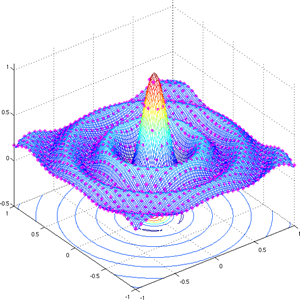
\includegraphics[scale=0.25]{../../img/sinc.PNG}}
\begin{definition}
设\(V_{1},\ldots ,V_{m}\)均为\(\mathbf{F}\)上的向量空间。

\begin{enumerate}
\item 定义积\(V_{1}\times \ldots \times V_{m}\)为:\[V_{1}\times \ldots \times V_{m} = \{(v_{1},\ldots ,v_{m}):v_{1}\in V_{1},\ldots ,v_{m}\in V_{m}\}\]
\item 定义\(V_{1}\times \ldots \times V_{m}\)上的加法为:\[(u_{1},\ldots ,u_{m}) + (v_{1},\ldots ,v_{m}) = (u_{1}+v_{1},\ldots ,u_{m}+v_{m})\]
\item 定义\(V_{1}\times \ldots \times V_{m}\)上的标量乘法为\[\lambda (v_{1},\ldots ,v_{m}) = (\lambda v_{1}, \lambda v_{2}, \ldots ,\lambda v_{m})\]
\end{enumerate}
\end{definition}

显然,向量空间的积也是向量空间,我们只需要证明其满足齐次可加性,并且零元也位于这个空间即可。

\begin{instance}
\(\mathcal{P}_{2}( \mathbf{R}) \times \mathbf{R}^{3}\)中的元素是长度为\(2\)的组,组的第一项是\(\mathcal{P}_{2}( \mathbf{R})\)中的元素,组的第二项是\(\mathbf{R}^{3}\)中的元素。比如\((5-6x+x^{2},(5,8,6))\in \mathcal{P}_{2}( \mathbf{R}) \times \mathbf{R}^{3}\)
\end{instance}

\begin{instance}
\(\mathbf{R}^{2}\times \mathbf{R}^{3}\)等于\(\mathbf{R}^{5}\)么? \(\mathbf{R}^{2}\times \mathbf{R}^{3}\)与\(\mathbf{R}^{5}\)同构么?

首先根据定义,\(\mathbf{R}^{2}\times \mathbf{R}^{3} = ((x_1,x_2),(x_3,x_4,x_5))\),其中\(x_{1},x_{2},x_{3},x_{4},x_{5}\in \mathbf{R}\) 而\(\mathbf{R}^{5}\)中的元素为\((x_{1},x_{2},x_{3},x_{4},x_{5})\)

\(\mathbf{R}^{2}\times \mathbf{R}^{3}\)和\(\mathbf{R}^{5}\)看起来很像,但是这两个集合是不相等的,因为\(\mathbf{R}^{2}\times \mathbf{R}^{3}\) 中的元素是二元组,其中第一个元素是个二元组,第二个元素是三元组,而\(\mathbf{R}^{5}\)中的元素是五元组,每一个元素都是实数。

但是\(\mathbf{R}^{2}\times \mathbf{R}^{3}\)与\(\mathbf{R}^{5}\)显然是同构的,从\(\mathbf{R}^{2}\times \mathbf{R}^{3}\)到\(\mathbf{R}^{5}\)的映射既单又满。
\end{instance}

\begin{instance}
求\(\mathcal{P}_{2}{ (\mathbf{R})}\times \mathbf{R}^{2}\)的一个基。

有:
\[(1,(0,0)),(x,(0,0)),(x^{2},(0,0)),(0,(1,0)),(0,(1,0))\]
\end{instance}
推广上面的这个例子,我们有:
\begin{theorem}
设\(V_{1},\ldots ,V_{m}\)均为有限维向量空间,则\(V_{1}\times \ldots \times V_{m}\)是有限维的,且:
\[\dim(V_{1}\times \ldots \times V_{m}) = \dim V_{1} + \ldots + \dim V_{m}\]
\end{theorem}
\begin{proof}
我们可以选取每个\(V_{j}\)的一个基。对于每个\(V_{j}\)的每个基向量,考虑\(V_{1}\times \ldots \times V_{m}\)的如下元素:第\(j\)个位置为此基向量,其余位置为\(0\)。显然所有这些向量构成的组是线性无关的,且张成\(V_{1}\times \ldots \times V_{m}\),因此是\(V_{1}\times \ldots \times V_{m}\)的基。这个基的长度是\(\dim V_{1} + \ldots + \dim V_{m}\)
\end{proof}

接下来我们考虑积与直和的关系
\begin{theorem}
设\(U_{1},\ldots ,U_{m}\)均为\(V\)的子空间。线性映射:\(\Gamma: U_{1}\times \ldots \times U_{m}\rightarrow U_{1} + \ldots +U_{m}\) 定义为:\(\Gamma(u_{1},\ldots ,u_{m}) = u_{1} + \ldots + u_{m}\),则\(U_{1} + \ldots + U_{m}\)是直和当且仅当\(\Gamma\)是单射。
\end{theorem}

\begin{proof}
线性映射\(\Gamma\)是单的当且仅当\(0\)表示为\(u_{1} + \ldots + u_{m}\)时,每个\(u_{j}\)都等于\(0\). 根据直和的条件,我们知道线性映射\(\Gamma\)是单的与\(U_{1}+ \ldots + U_{m}\)是直和这两个命题是等价的。
\end{proof}

\begin{theorem}
设\(V\)是有限维的,\(U_{1},\ldots ,U_{m}\)是\(V\)的子空间,则\(U_{1} + \ldots U_{m}\)是直和当且仅当\(\dim(U_{1} + \ldots + U_{m}) = \dim U_{1} + \ldots + \dim U_{m}\)
\end{theorem}

\begin{proof}
定义线性映射:\(\Gamma: U_{1}\times \ldots \times U_{m}\rightarrow U_{1} + \ldots +U_{m}\) 定义为:\(\Gamma(u_{1},\ldots ,u_{m}) = u_{1} + \ldots + u_{m}\)。 当线性映射\(\Gamma\)是单的时,根据线性映射基本定理有\(\dim(U_{1} +\ldots + U_{m}) = \dim(U_{1}\times \ldots \times U_{m})\)

又因为\(\dim(U_{1}\times \ldots \times U_{m}) = \dim(U_{1}) + \ldots + \dim(U_{m})\),所以必有:
\(\dim(U_{1} + \ldots + U_{m}) = \dim U_{1} + \ldots + \dim U_{m}\)
\end{proof}



首先定义向量与子空间的和,然后定义商空间。

\begin{definition}
设\(v\in V\),\(U\)是\(V\)的子空间,则\(v+U\)是\(V\)的子集,定义如下:
\begin{equation}
\label{eq:1}
v+U = \{v+u:u\in U\}
\end{equation}
\end{definition}

\begin{definition}
\begin{enumerate}
\item \(V\)的仿射子集是\(V\)的形如\(v+U\)的子集,其中\(v\in V\),\(U\)是\(V\)的子空间。
\item 对于\(v\in V\)和\(V\)的子空间\(U\),称仿射子集\(v+U\)平行于\(U\)
\end{enumerate}
\end{definition}

\begin{instance}
若\(U=\{(x,y,0)\in \mathbf{R}^{3}:x,y\in \mathbf{R}\}\)则\(\mathbf{R}^{3}\)的平行于\(U\)的仿射子集是\(\mathbf{R}^{3}\)中在通常意义下平行于\(xy\)平面\(U\)的那些平面(注意这里必须是平面,直线不行.)。
\end{instance}

\begin{definition}
设\(U\)是\(V\)的子空间,则商空间\(V/U\)是指\(V\)中所有平行于\(U\)的仿射子集的集合。也就是说:
\begin{equation}
\label{eq:2}
V/U = \{v+U:v\in V\}
\end{equation}
\end{definition}

\begin{instance}
\begin{enumerate}
\item 若\(U = \{(x,2x)\in \mathbf{R}^{2}:x\in \mathbf{R}\}\),则\(\mathbf{R}^{2}/U\)是\(\mathbf{R}^{2}\)中所有平行于\(U\)的直线的集合。
\item 若\(U\)是\(\mathbf{R}^{3}\)中的包含原点的直线,则\(\mathbf{R}^{3}/U\)是\(\mathbf{R}^{3}\)中所有平行于\(U\)的直线的集合。
\item 若\(U\)是\(\mathbf{R}^{3}\)中的包含原点的平面,则\(\mathbf{R}^{3}/U\)是\(\mathbf{R}^{3}\)中所有平行于\(U\)的平面的集合。
\end{enumerate}
\end{instance}

\begin{theorem}
设\(U\)是\(V\)的子空间,\(v,w\in V\),则一下陈述等价:
\begin{enumerate}
\item \(v-w \in U\)
\item \(v+U = w+U\)
\item \((v+U)\cap (w+U) \neq \varnothing\)
\end{enumerate}
\end{theorem}

\begin{proof}
假设1成立,则有对于任何的\(u\in U\)都有:
\begin{equation}
\label{eq:3}
v+ u = w + v-w +u = w + (v-w) +u \in w + U
\end{equation}
所以\(v+U\subseteq w + U\)

对于所有的\(u in U\)都有:
\begin{equation}
\label{eq:4}
(w+u) = v+w -v +u = v + (w-v) + u \in v + U
\end{equation}
所以\(w+U\subseteq v + U\)

从2到3是显然的。

我们证明从3到1. 假设\((v+U)\cap (w+U) \neq \varnothing\) ,则存在\(u_{1},u_{2}\)使得:
\begin{equation}
\label{eq:5}
v+u_{1} = w + u_{2}
\end{equation}
所以有\(v-w = u_{2} - u_{1}\),显然有\(v-w\in U\)
\end{proof}

\begin{definition}
定义\(V/U\)上的加法和标量乘法。设\(U\)是\(V\)的子空间,则\(V/U\)上的加法和标量乘法定义为:对任意\(v,w\in V\)和\(\lambda \in \mathbf{F}\):
\begin{eqnarray}
\label{eq:6}
(v+U)+(w+U)&=&(v+W) + U \\
\lambda(v+U) &=&(\lambda v) + U
\end{eqnarray}
\end{definition}

\begin{theorem}
设\(U\)是\(V\)的子空间。则\(V/U\)按照上面定义的加法和标量乘法构成向量空间。
\end{theorem}

\begin{proof}
在我们定义\(V/U\)的加法和标量乘法中,一个问题是平行于\(U\)的仿射子集的表示并不是唯一的。具体来说,设\(v,w\in V\),假设\(\hat{v},\hat{w}\in V\)使得\(v+U = \hat{v} + U\)和\(w +U = \hat{w} + U\),要证明上面给出的\(V/U\)上的加法是有意义的,必须证明\((v+w) + U = (\hat{v} + \hat{w}) + U\)

因为\(v-\hat{v}\in U\), \(w- \hat{w} \in U\),因为\(U\)是\(V\)的子空间,所以在加法下封闭,所以\(v- \hat{v} + w - \hat{w} \in U\)所以\(v + w - ( \hat{v} + \hat{w}) \in U\),所以有:
\begin{equation}
\label{eq:7}
v + w + U = \hat{v} + \hat{w} + U
\end{equation}

同理,设\(\lambda \in \mathbf{F}\),因为\(U\)是\(V\)的子空间,所以在标量乘法下封闭从而有\(\lambda (v - \hat{v})\in U\),所以有:
\begin{equation}
\label{eq:8}
\lambda v + U = \lambda \hat{v} + U
\end{equation}

现在我们假设\(v+U,u+U\in V/U\),则有\(v+U + u + U = (v+u) + U\in V/U\),同理\(\lambda \in \mathbf{F}\)则\(\lambda (v + U) = \lambda v + U \in V/U\)

另外\(V/U\)中的加法零元是\(U\).因为任何的\(v+U\)在加上\(U\)都是其本身。
\end{proof}

\begin{definition}
设\(U\)是\(V\)的子空间. 商映射\(\pi\)是如下定义的线性映射\(\pi :V\rightarrow V/U\)对任意的\(v\in V\)满足:\(\pi(v) = v+U\)
\end{definition}

\begin{theorem}
设\(V\)是有限维的,\(U\)是\(V\)的子空间,则:\(\dim V/U = \dim V - \dim U\)
\end{theorem}

\begin{proof}
定义\(\pi : V\rightarrow V/U\),则有\(null\pi = U\),根据线性映射基本定理则有:
\begin{equation}
\label{eq:9}
\dim V = \dim null\pi + \dim range \pi
\end{equation}
因为\(range\pi = V/U\),所以\(\dim V/U = \dim V - \dim U\).
\end{proof}

从商映射的一般形式可以推导出一个特别重要映射。
\begin{definition}
设\(T\in \mathcal{L}(V,W)\),定义\(\tilde{T}:V/(nullT) \rightarrow W\),如下:
\begin{equation}
\label{eq:10}
\tilde{T}(v + nullT) = Tv
\end{equation}
\end{definition}

现在对这个定义做一下简单的说明。设\(u,v\in V\)使得\(u+nullT = v+ nullT\)则有\(u-v\in nullT\),于是\(T(u-v) = 0\),则\(Tu=Tv\),因此\(\tilde{T}\)的定义是有意义的。

\begin{theorem}
设\(T\in \mathcal{L}(V,W)\),则:
\begin{enumerate}
\item \(\tilde{T}\)是\(V/(nullT)\)到\(W\)的线性映射;
\item \(\tilde{T}\)是单的。
\item \(range \tilde{T} = range T\)
\item \(V/nullT\)同构于\(rangeT\)
\end{enumerate}
\end{theorem}
\end{document}
